\chapter{Circuiti}

\section{Esercizio 1}

\subsection{Prima domanda}

\begin{center}
  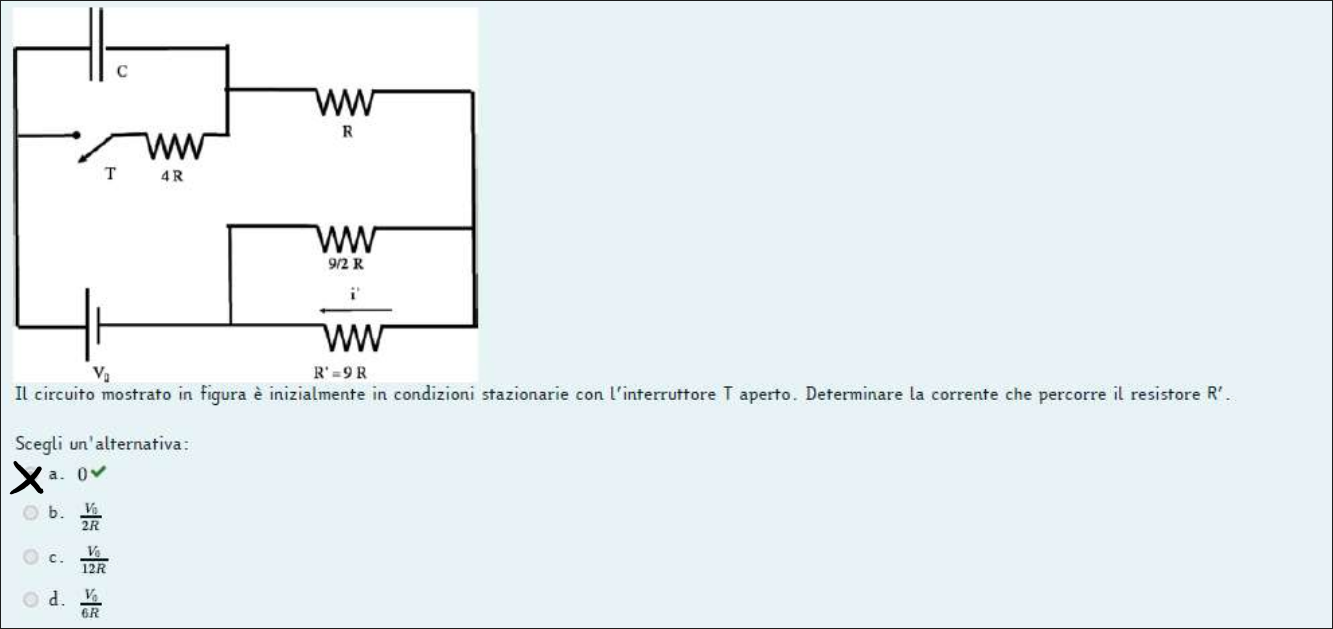
\includegraphics[scale=0.34]{es1-1c.png}
\end{center}

\paragraph{Risposta:} un condensatore carico, in condizioni stazionarie si comporta come un circuito aperto. Perciò, essendo aperto anche l'interruttore, nella resistenza non passa corrente. 

\subsection{Seconda domanda}

\begin{center}
  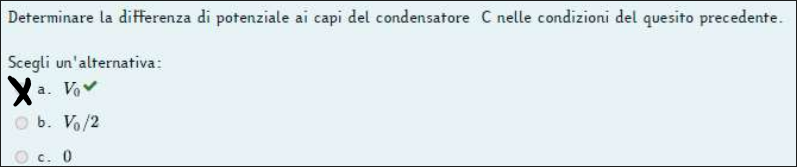
\includegraphics[scale=0.34]{es1-2c.png}
\end{center}

\paragraph{Risposta:} dal lato sinistro è collegato direttamente alla batteria ($V_0$) mentre dal lato destro non passa corrente, come specificato nella risposta precedente. 

\subsection{Terza domanda}

\begin{center}
  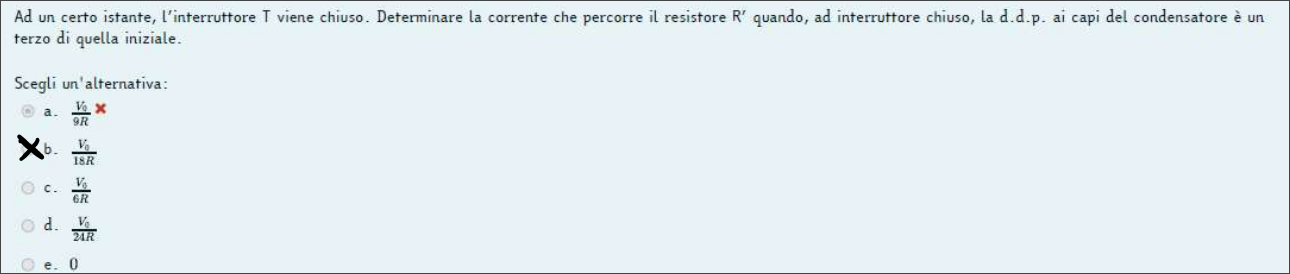
\includegraphics[scale=0.34]{es1-3c.png}
\end{center}

\paragraph{Risposta:} si usa Kirchoff. Il condensatore viene considerato come una f.e.m. con verso positivo contrario alla corrente. 

\begin{equation}
  \begin{cases}
    I_1 = I_2 + I_3 \\
    V_0 - I_3 R - 4 I_1 R = 0\\
    \frac{1}{3} V_0 - I_3 R = 0
  \end{cases}
\end{equation}

$$I_1 = \frac{V_0}{6}$$

$$I(R') = \frac{V_0}{6} \frac{2}{9}$$

\section{Esercizio 2}

\subsection{Prima domanda}

\begin{center}
  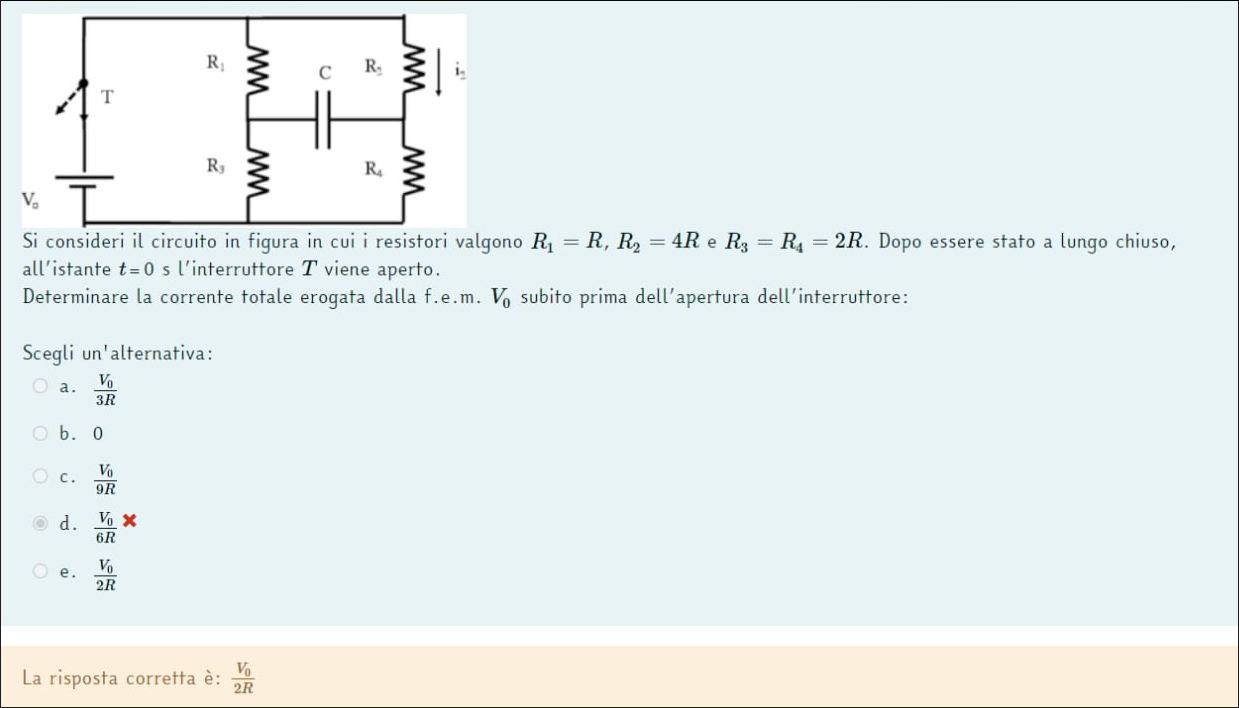
\includegraphics[scale=0.34]{es2-1c.png}
\end{center}

\paragraph{Risposta:} in condizioni di stazionarietà con l'interruttore chiuso il condensatore è un circuito aperto, quindi occorre solamente calcolare le resistenze in serie e in parallelo. 

$$R_{1-3} = R_1 + R_3 = 3 R$$

$$R_{2-4} = R_2 + R_4 = 6 R$$

$$R_T = 2R$$ 

$$i = \frac{V}{R_T} = \frac{V_0}{2R}$$

\subsection{Seconda domanda}

\begin{center}
  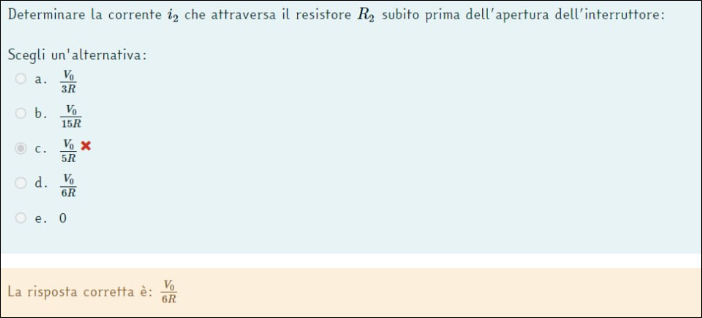
\includegraphics[scale=0.4]{es2-2c.png}
\end{center}

\paragraph{Risposta:} ???

\subsection{Terza domanda}

\begin{center}
  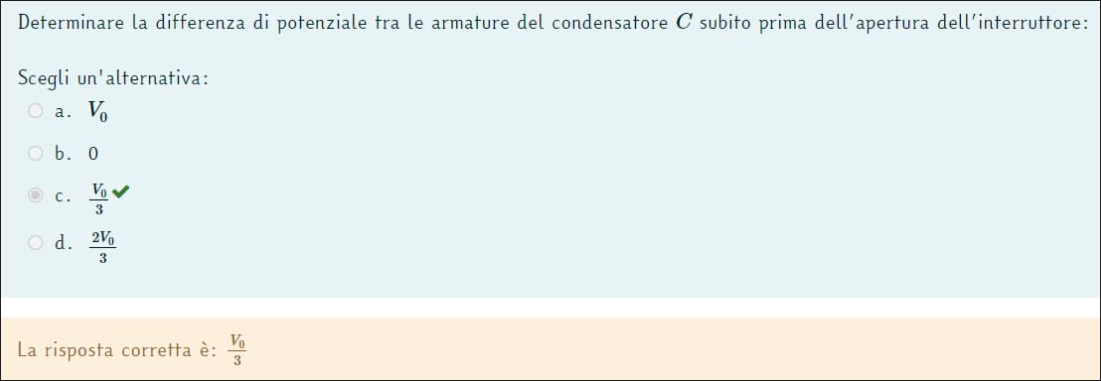
\includegraphics[scale=0.4]{es2-3c.png}
\end{center}

